\chapter{Resultados Experimentais e Discussões}
Neste capítulo serão expostos os resultados das medidas realizadas conforme os métodos e procedimentos elencados no capítulo anterior, será realizado uma descrição do resultado e juntamente será feito uma discussão acerca deste.

\section{Resultados da Caracterização da Resposta em Frequência}
Os gráficos com as respostas em frequência de cada NFP em sua versão com e sem plano de terra esta exposto no apêndice. Neste capítulo deixamos os gráficos que condensam as respostas de todas as NFPs de mesmo tamanho, porém em alguns momentos remeteremos os comentários aos gráficos expostos no apêndice.

\begin{figure}[htb!]
	\centering 
	\caption{Resposta em Frequência - FX05XT}
	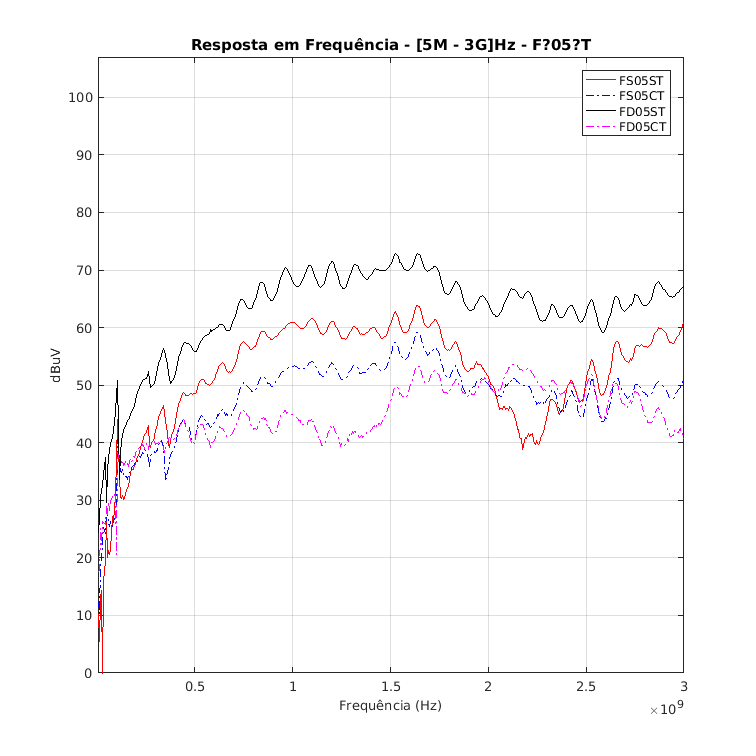
\includegraphics[scale=0.7]{./img/FX05XT}
	\fonte{Elaborado pelo Autor (2019)}
	%\legend{\hspace{-218pt}Fonte:~\citeonline[p.~8]{paul2006}}
	\label{fig:FX05XT}
\end{figure}

Na figura~\ref{fig:FX05XT} visualizamos, de forma condensada, as curvas para a NFP de 0.5mm de raio nas versões em face simples e dupla, com e sem plano de terra (FS05ST, FS05CT, FD05ST e FD05CT respectivamente). Podemos notar inicialmente nesta figura que a NFP na versão face simples sem plano de terra (em vermelho) possui uma região de resposta constante em $dB \mu V$ em uma faixa de frequência que vai de aproximadamente 900MHz à 1.75GHz, enquanto que sua versão face simples com plano de terra (em azul) ocorre um aumento significativo nessa faixa de frequência, em apêndice na figura~\ref{fig:FS05XT} podemos visualizar apenas essas duas curvas. Na versão em face dupla sem o plano de terra (em negro), notamos nitidamente que a sensibilidade em $dB \mu V$ aumenta na ordem de 10 $dB \mu V$, isso se deve ao fato de termos agora dois laços, um em cada face da PCI e novamente notamos (em magenta) que a inclusão do plano de terra, agora em face dupla, suaviza a resposta e aumenta a faixa de frequência que tem uma resposta constante em $dB \mu V$, em apêndice na figura~\ref{fig:FD05XT} podemos visualizar as curvas para as NFPs de face dupla. 

Na figura~\ref{fig:FX10XT} visualizamos, de forma condensada, as curvas para a NFP de 1mm de raio nas versões em face simples e dupla, com e sem plano de terra (FS10ST, FS10CT, FD10ST e FD10CT respectivamente). Podemos notar inicialmente nesta figura que a NFP na versão face simples sem plano de terra (em vermelho) possui uma região de resposta constante em $dB \mu V$ em uma faixa de frequência que vai de aproximadamente 900MHz à 1.75GHz, similar a NFP anterior, nessa versão notamos também que e em 2.2GHz há uma singularidade, %onde $\omega_0 = \frac{1}{\sqrt{L_oC_o}}$ uma ressonância. 
Na versão face simples com plano de terra (em azul) notamos o suprimento dessa singularidade, haja vista que o plano de terra inclui uma capacitância de acoplamento que modifica a resposta do circuito equivalente da NFP. No apêndice na figura~\ref{fig:FS10XT} podemos visualizar apenas essas duas curvas (FS10ST e FS10CT). Na versão em face dupla sem o plano de terra (em negro), notamos um pequeno aumento na sensibilidade, isso se deve ao fato de termos agora dois laços, um em cada face da PCI e novamente notamos (em magenta) que a inclusão do plano de terra, agora em face dupla, suaviza a resposta e aumenta a faixa de frequência que tem uma resposta constante em $dB \mu V$. De todas as versões desta NFP de 1mm, a versão dupla face com plano de terra é a que deu o melhor resultado, mesmo sendo menos sensitiva. Em apêndice na figura~\ref{fig:FD10XT} podemos visualizar as curvas para as NFPs de face dupla.
\begin{figure}[htb!]
	\centering 
	\caption{Resposta em Frequência - FX10XT}
	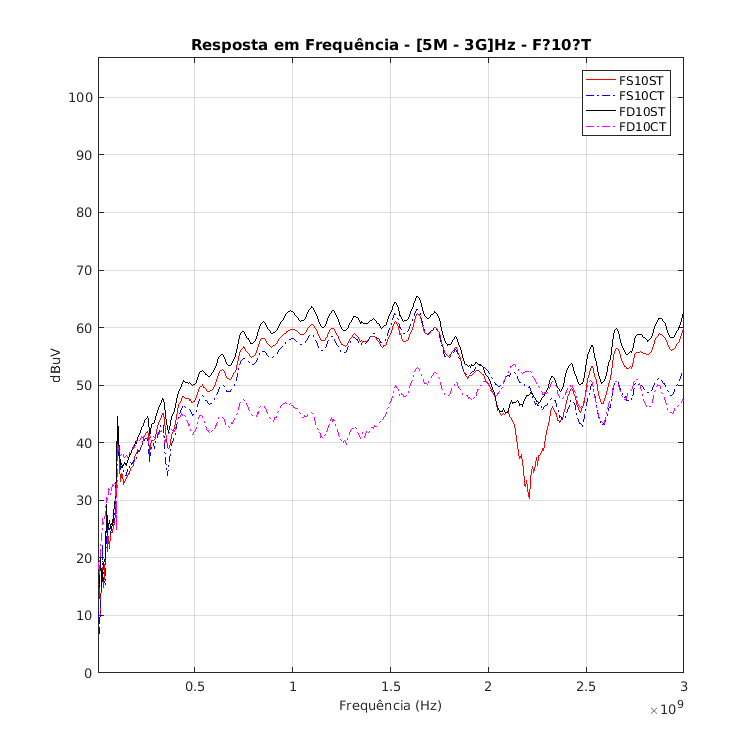
\includegraphics[scale=0.7]{./img/FX10XT}
	\fonte{Elaborado pelo Autor (2019)}
	%\legend{\hspace{-218pt}Fonte:~\citeonline[p.~8]{paul2006}}
	\label{fig:FX10XT}
\end{figure} 

\begin{figure}[htb!]
	\centering 
	\caption{Resposta em Frequência - FX15XT}
	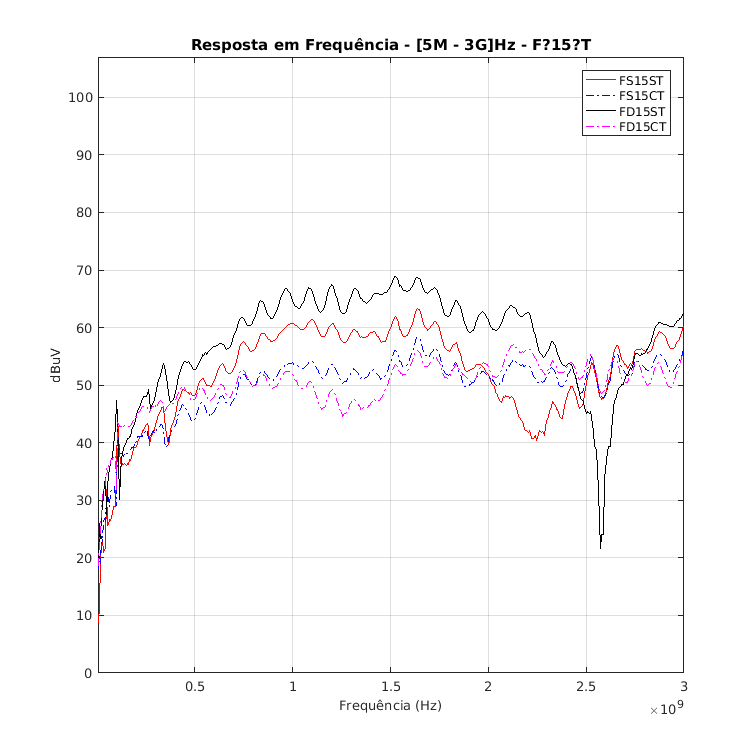
\includegraphics[scale=0.7]{./img/FX15XT}
	\fonte{Elaborado pelo Autor (2019)}
	%\legend{\hspace{-218pt}Fonte:~\citeonline[p.~8]{paul2006}}
	\label{fig:FX15XT}
\end{figure}

Na figura~\ref{fig:FX15XT} visualizamos, de forma condensada, as curvas para a NFP de 1.5mm de raio nas versões em face simples e dupla, com e sem plano de terra (FS15ST, FS15CT, FD15ST e FD15CT respectivamente). Podemos notar inicialmente nesta figura que a NFP na versão face simples sem plano de terra (em vermelho) possui uma região de resposta constante em $dB \mu V$ em uma faixa de frequência que vai de aproximadamente 900MHz à 1.75GHz, mantendo a similaridade com as anteriores. Na versão face simples com plano de terra (em azul) notamos uma aumento significativo da faixa onde há uma resposta constante em $dB \mu V$, haja vista que o plano de terra inclui uma capacitância de acoplamento que modifica a resposta do circuito equivalente da NFP. No apêndice na figura~\ref{fig:FS15XT} podemos visualizar apenas essas duas curvas (FS10ST e FS10CT). Na versão em face dupla sem o plano de terra (em negro), notamos um pequeno aumento na sensibilidade, isso se deve ao fato de termos agora dois laços, um em cada face da PCI, nessa versão notamos mais nitidamente uma singularidade, agora próximo de 2.6GHz e novamente notamos (em magenta) que a inclusão do plano de terra, agora em face dupla, elimina esta singularidade, suaviza a resposta e aumenta a faixa de frequência que tem uma resposta constante em $dB \mu V$. De todas as versões desta NFP de 1.5mm, a versão dupla face com plano de terra é a que deu o melhor resultado, mesmo sendo menos sensitiva. Em apêndice na figura~\ref{fig:FD15XT} podemos visualizar as curvas para as NFPs de face dupla.

\begin{figure}[htb!]
	\centering 
	\caption{Resposta em Frequência - FX30XT}
	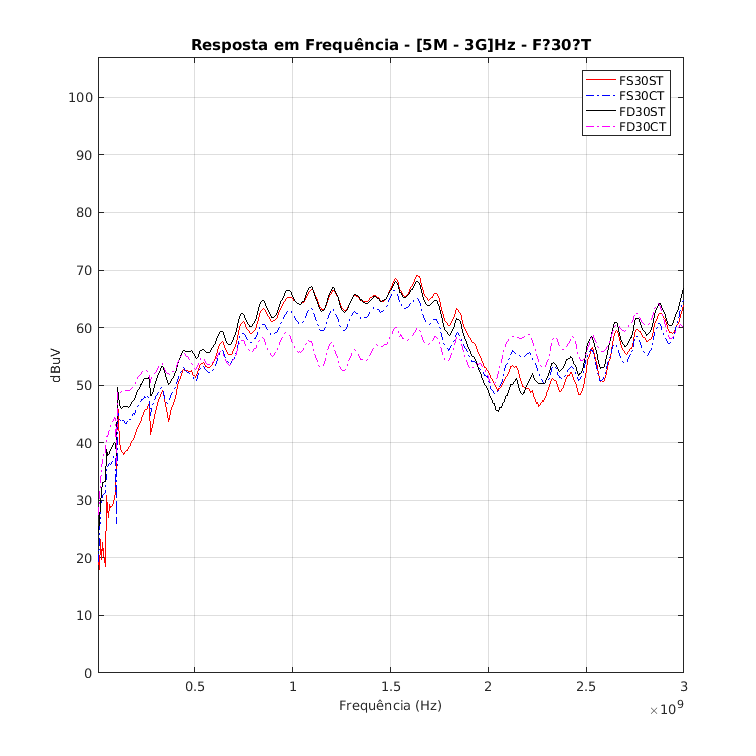
\includegraphics[scale=0.7]{./img/FX30XT}
	\fonte{Elaborado pelo Autor (2019)}
	%\legend{\hspace{-218pt}Fonte:~\citeonline[p.~8]{paul2006}}
	\label{fig:FX30XT}
\end{figure}

Na figura~\ref{fig:FX30XT} visualizamos, de forma condensada, as curvas para a NFP de 3mm de raio nas versões em face simples e dupla, com e sem plano de terra (FS30ST, FS30CT, FD30ST e FD30CT respectivamente). Notamos que as versões desta NFP em face simples com e sem plano de terra e face dupla sem plano de terra, apresentam respostas muito similares, possuindo uma região de resposta constante em $dB \mu V$ em uma faixa de frequência que vai de aproximadamente 900MHz à 1.75GHz. Somente na versão face dupla com plano de terra é que notamos uma diferença mais significativo, novamente o plano de terra suavisa a resposta, diminui a sensibilidade porém aumenta a faixa de resposta constante em $dB \mu V$. No apêndice nas figuras~\ref{fig:FS30XT} e ~\ref{fig:FD30XT} podemos visualizar as curvas de forma separada.

\begin{figure}[htb!]
	\centering 
	\caption{Resposta em Frequência - FX60XT}
	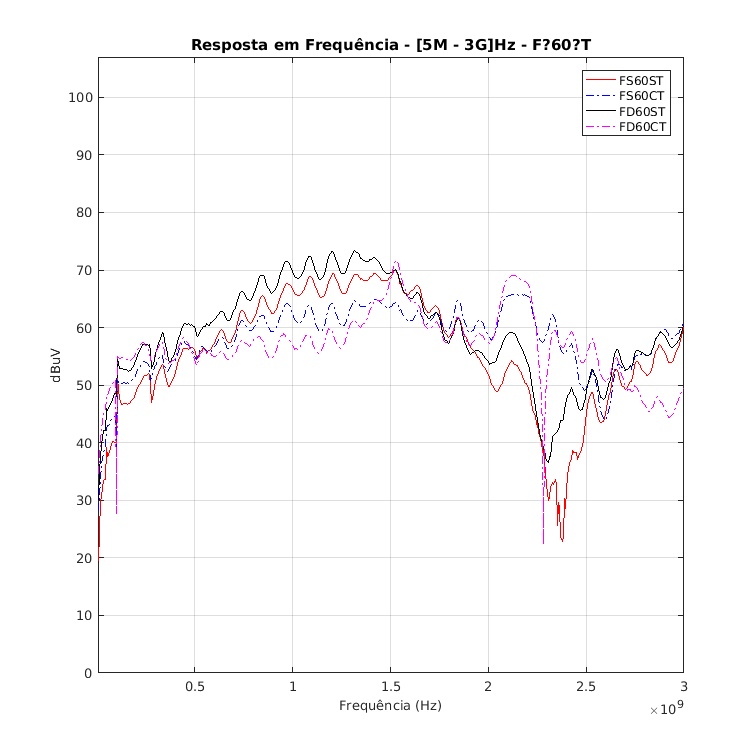
\includegraphics[scale=0.7]{./img/FX60XT}
	\fonte{Elaborado pelo Autor (2019)}
	%\legend{\hspace{-218pt}Fonte:~\citeonline[p.~8]{paul2006}}
	\label{fig:FX60XT}
\end{figure}

Na figura~\ref{fig:FX60XT} visualizamos, de forma condensada, as curvas para a NFP de 6mm de raio nas versões em face simples e dupla, com e sem plano de terra (FS60ST, FS60CT, FD60ST e FD60CT respectivamente). Notamos que as versões desta NFP em face simples e dupla sem plano de terra, apresentam respostas muito similares, possuindo uma região de resposta constante em $dB \mu V$ em uma faixa de frequência menor que as anteriores, que vai de aproximadamente 1GHz à 1.5GHz. Nas versões face simples e dupla com plano de terra, notamos que o plano de terra suavisa a resposta, diminui a sensibilidade porém aumenta a faixa de resposta constante em $dB \mu V$. No apêndice nas figuras~\ref{fig:FS60XT} e ~\ref{fig:FD60XT} podemos visualizar as curvas de forma separada.

%###########################
%###########################

\section{Resultados da Caracterização da Intensidade por Distância}
Conforme o procedimento descrito no capítulo anterior, foi coletado para cada posição lateral (na direção do eixo y) o valor de intensidade em $dB \mu V$ nas frequências de 5MHz, 10MHz, 15MHz, 20MHz e 25MHz (limite máximo do gerador de função disponível). Será exposto agora os gráficos contendo o valor de tensão em $dB \mu V$ lido de cada NFP variando-se a posição lateral.

\begin{figure}[htb!]
	\centering
 	\caption{Intensidade por Distância - 5MHz}
	\subfloat[][NFPs Face Simples - 5MHz]{
		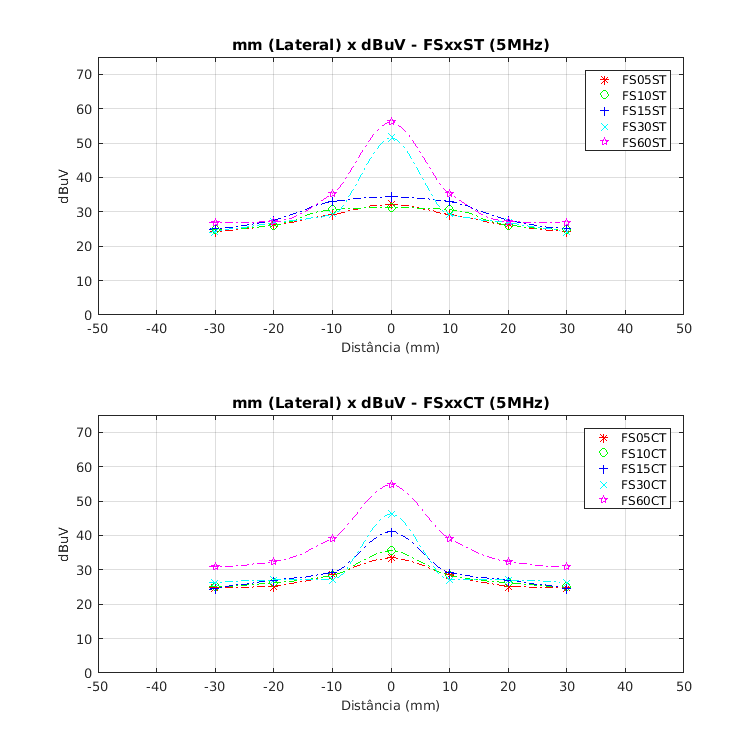
\includegraphics[scale=0.4]{./img/FSxxxT_5M}
		\label{fig:FSxxxT_5M}}
	\subfloat[][NFPs Face Dupla - 5MHz]{
		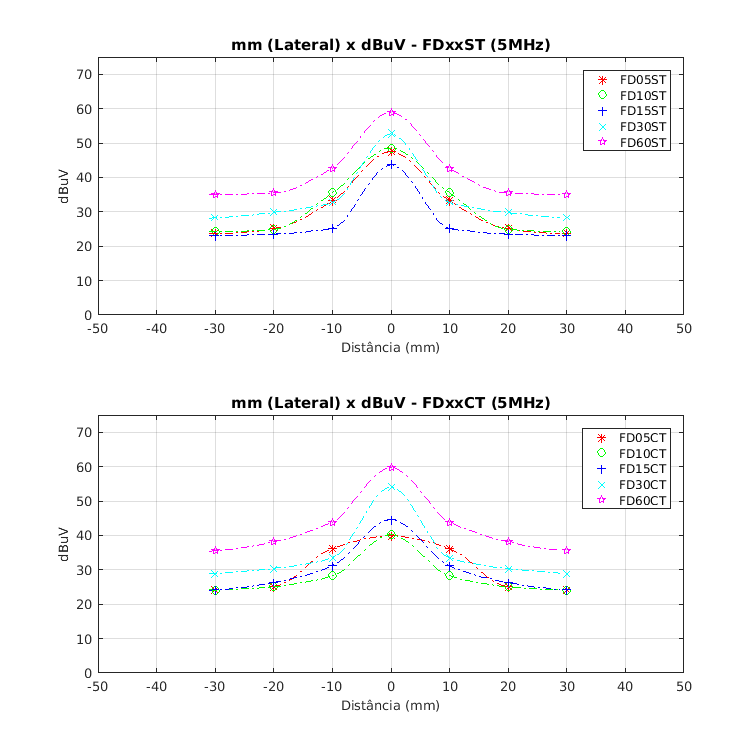
\includegraphics[scale=0.4]{./img/FDxxxT_5M}
		\label{fig:FDxxxT_5M}}
    \fonte{Elaborado pelo Autor (2019)}
\end{figure}

Na figura~\ref{fig:FSxxxT_5M} vemos os gráficos na frequência de 5MHz de todas as versões em face simples, sem e com plano de terra. Nesta imagem, no primeiro quadro, exceto as versões FS30ST e FS60ST, todas as demais tem baixa sensibilidade e pouca resolução espacial, somente as versões FS30ST e FS60ST, que já possuem um raio maior que 1.5mm são as que apresentam uma boa sensibilidade nesta frequência. No segundo quadro da figura~\ref{fig:FSxxxT_5M}, com a inclusão do plano de terra, notamos que todas as versões melhoram sua sensibilidade, e notamos também que a versão FD60CT perde resolução espacial, haja vista que para todas as posições avaliadas esta versão possui um nível de tensão em $dB \mu V$ maior que as demais. 

Na figura~\ref{fig:FDxxxT_5M} vemos os gráficos na frequência de 5MHz de todas as versões em face dupla, sem e com plano de terra. Notamos no primeiro quadro desta imagem que o acréscimo de mais uma volta de espira aumente a sensibilidade para todas as versões de NFPs avaliadas, sendo que a que possui a melhor resolução espacial, nesta frequência é a FD15ST, mesmo sendo a menos sensitiva. No segundo quadro da figura~\ref{fig:FDxxxT_5M} notamos que a inclusão do plano de terra, para esta frequência, não melhora a resolução espacial e não influência de forma significativa a sensibilidade. Dessa forma, o melhor resultado em termos de resolução espacial, nesta frequência (5MHz) é a versão FD15ST.

\begin{figure}[htb!]
	\centering
 	\caption{Intensidade por Distância - 10MHz}
	\subfloat[][NFPs Face Simples - 10MHz]{
		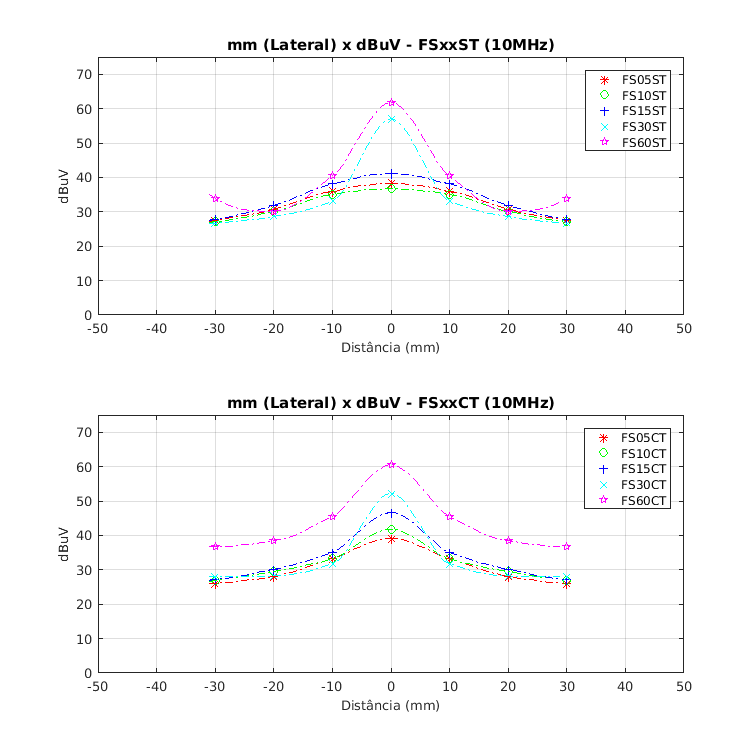
\includegraphics[scale=0.4]{./img/FSxxxT_10M}
		\label{fig:FSxxxT_10M}}
	\subfloat[][NFPs Face Dupla - 10MHz]{
		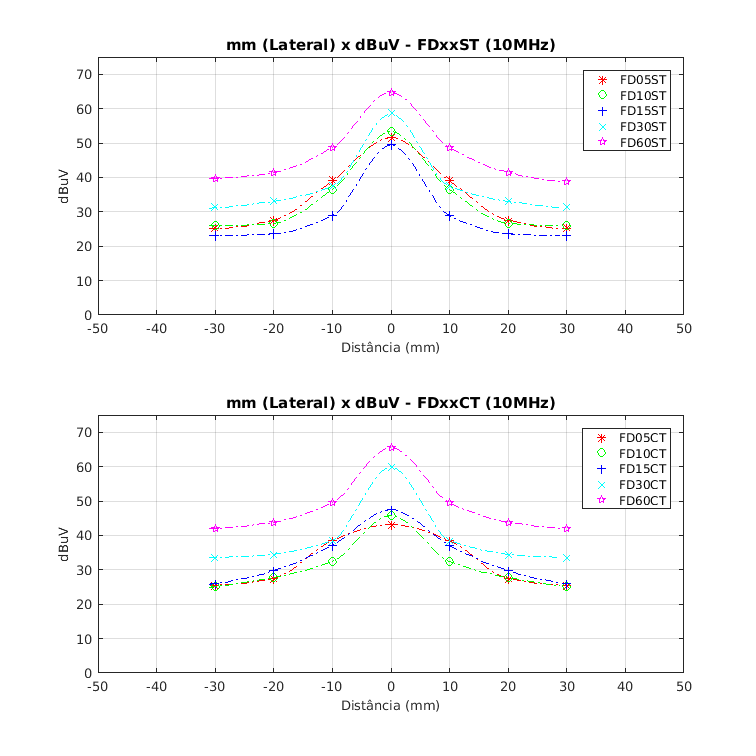
\includegraphics[scale=0.4]{./img/FDxxxT_10M}
		\label{fig:FDxxxT_10M}}
    \fonte{Elaborado pelo Autor (2019)}
\end{figure}

Na figura~\ref{fig:FSxxxT_10M} vemos os gráficos na frequência de 10MHz de todas as versões em face simples, sem e com plano de terra. Nesta imagem, no primeiro quadro, exceto as versões FS30ST e FS60ST, todas as demais tem baixa sensibilidade e pouco resolução espacial, somente as versões FS30ST e FS60ST, que já possuem um raio maior que 1.5mm são as que apresentam uma boa sensibilidade nesta frequência. No segundo quadro da figura~\ref{fig:FSxxxT_5M}, com a inclusão do plano de terra, notamos que todas as versões melhoram sua sensibilidade, e notamos também que a versão FD60CT perde resolução espacial, haja vista que para todas as posições avaliadas esta versão possui um nível de tensão em $dB \mu V$ maior que as demais. 

Na figura~\ref{fig:FDxxxT_10M} vemos os gráficos na frequência de 10MHz de todas as versões em face dupla, sem e com plano de terra. Notamos no primeiro quadro desta imagem que o acréscimo de mais uma volta de espira aumente a sensibilidade para todas as versões de NFP avaliada, sendo que a que possui a melhor resolução espacial, nesta frequência é a FD15ST, mesmo sendo a menos sensitiva. No segundo quadro da figura~\ref{fig:FDxxxT_5M} notamos que a inclusão do plano de terra, para esta frequência, não melhora a resolução espacial e não influência de forma significativa a sensibilidade. Dessa forma, o melhor resultado em termos de resolução espacial, nesta frequência (10MHz), assim como foi para 5MHZ, é a versão FD15ST.

\begin{figure}[htb!]
	\centering
 	\caption{Intensidade por Distância - 15MHz}
	\subfloat[][NFPs Face Simples - 15MHz]{
		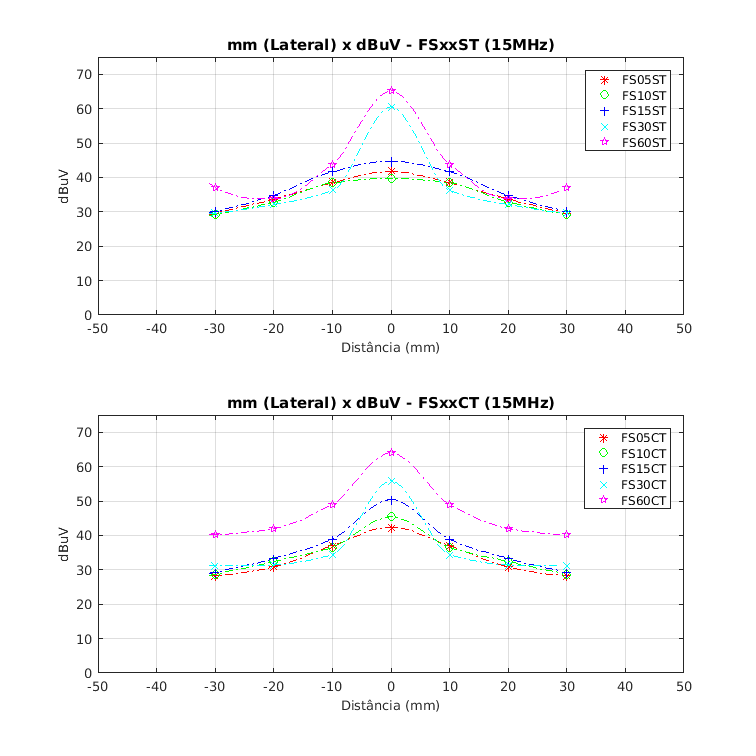
\includegraphics[scale=0.4]{./img/FSxxxT_15M}
		\label{fig:FSxxxT_15M}}
	\subfloat[][NFPs Face Dupla - 15MHz]{
		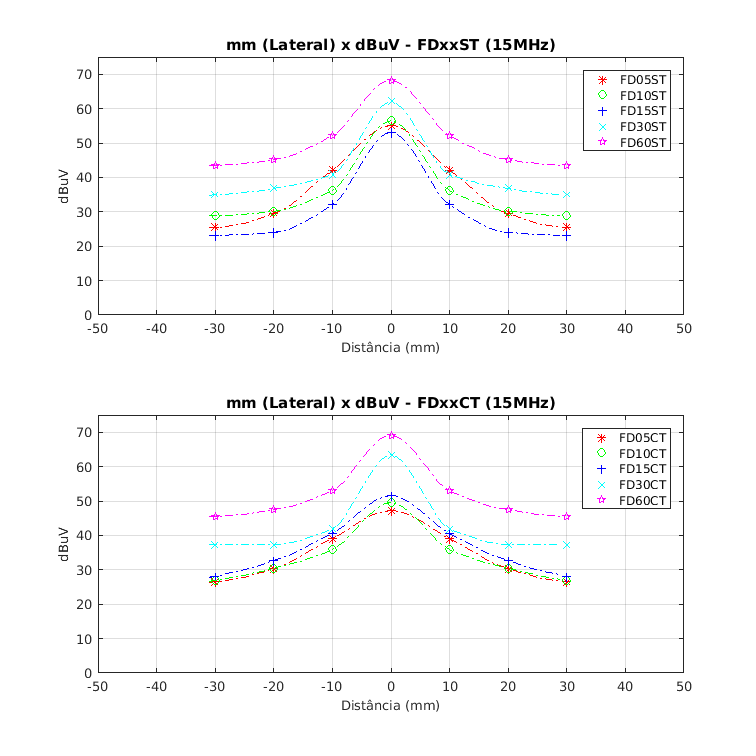
\includegraphics[scale=0.4]{./img/FDxxxT_15M}
		\label{fig:FDxxxT_15M}}
    \fonte{Elaborado pelo Autor (2019)}
\end{figure}

Na figura~\ref{fig:FSxxxT_15M} vemos os gráficos na frequência de 15MHz de todas as versões em face simples, sem e com plano de terra. Nesta imagem, no primeiro quadro, exceto as versões FS30ST e FS60ST, todas as demais tem baixa sensibilidade e pouca resolução espacial, somente as versões FS30ST e FS60ST, que já possuem um raio maior que 1.5mm são as que apresentam uma boa sensibilidade nesta frequência. No segundo quadro da figura~\ref{fig:FSxxxT_15M}, com a inclusão do plano de terra, notamos que todas as versões melhoram sua sensibilidade, e notamos também que a versão FD60CT perde resolução espacial, haja vista que para todas as posições avaliadas esta versão possui um nível de tensão em $dB \mu V$ maior que as demais. 

Na figura~\ref{fig:FDxxxT_15M} vemos os gráficos na frequência de 15MHz de todas as versões em face dupla, sem e com plano de terra. Notamos no primeiro quadro desta imagem que o acréscimo de mais uma volta de espira aumente a sensibilidade para todas as versões de NFP avaliada, sendo que a que possui a melhor resolução espacial, nesta frequência, continuar sendo a FD15ST, mesmo tendo a menor sensibilidade. No segundo quadro da figura~\ref{fig:FDxxxT_15M} notamos que a inclusão do plano de terra, para esta frequência, não melhora a resolução espacial e não influência de forma significativa a sensibilidade. Dessa forma, o melhor resultado em termos de resolução espacial, nesta frequência (15MHz), assim como foi nas anteriores, é a versão FD15ST.

\begin{figure}[htb!]
	\centering
 	\caption{Intensidade por Distância - 20MHz}
	\subfloat[][NFPs Face Simples - 20MHz]{
		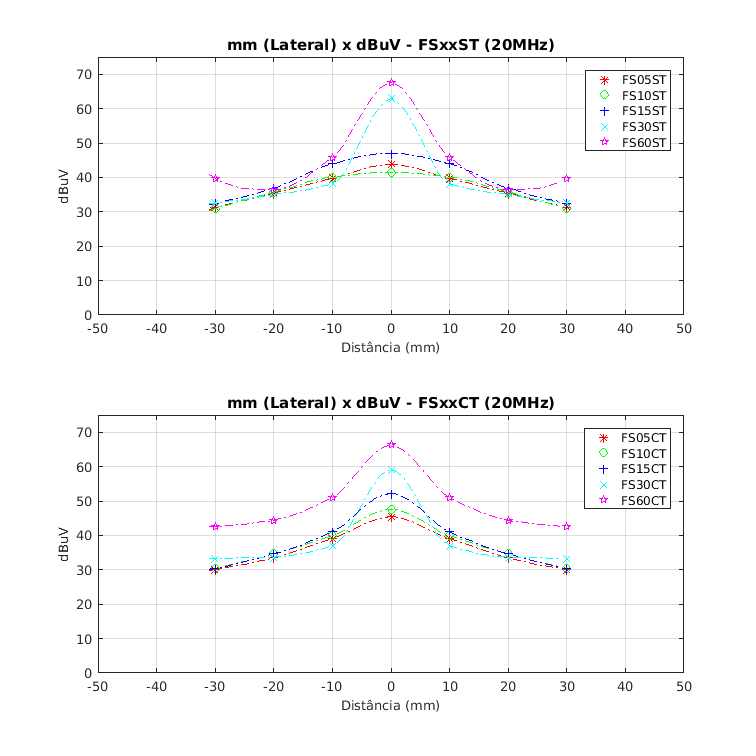
\includegraphics[scale=0.4]{./img/FSxxxT_20M}
		\label{fig:FSxxxT_20M}}
	\subfloat[][NFPs Face Dupla - 20MHz]{
		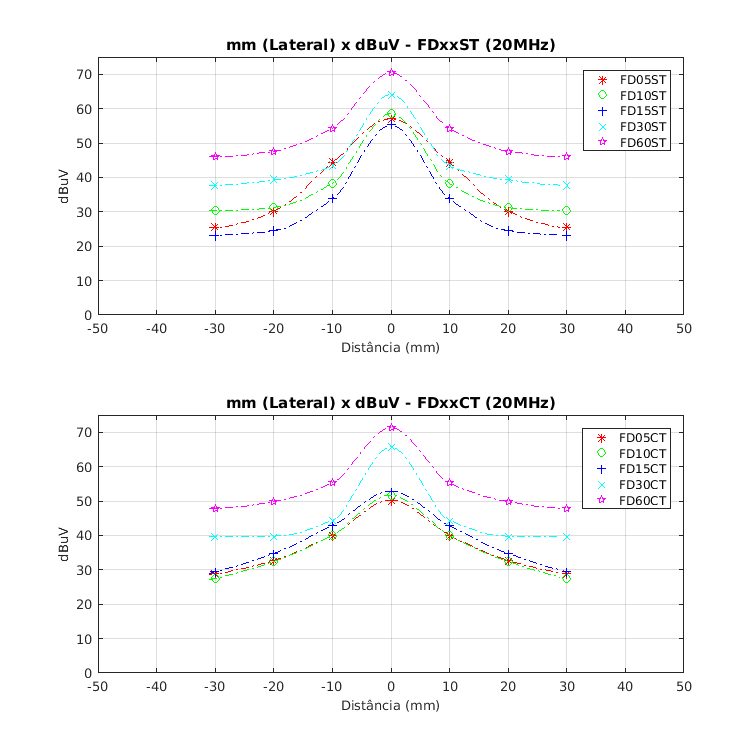
\includegraphics[scale=0.4]{./img/FDxxxT_20M}
		\label{fig:FDxxxT_20M}}
    \fonte{Elaborado pelo Autor (2019)}
\end{figure}

Na figura~\ref{fig:FSxxxT_20M} vemos os gráficos na frequência de 20MHz de todas as versões em face simples, sem e com plano de terra. Nesta imagem, no primeiro quadro, novamente exceto as versões FS30ST e FS60ST, todas as demais tem baixa sensibilidade e pouca resolução espacial, somente as versões FS30ST e FS60ST, que já possuem um raio maior que 1.5mm são as que apresentam uma boa sensibilidade nesta frequência. No segundo quadro da figura~\ref{fig:FSxxxT_20M}, com a inclusão do plano de terra, notamos que todas as versões melhoram sua sensibilidade, e notamos também que a versão FD60CT perde resolução espacial, haja vista que para todas as posições avaliadas esta versão possui um nível de tensão em $dB \mu V$ maior que as demais. 

Na figura~\ref{fig:FDxxxT_20M} vemos os gráficos na frequência de 20MHz de todas as versões em face dupla, sem e com plano de terra. Notamos no primeiro quadro desta imagem que o acréscimo de mais uma volta de espira aumente a sensibilidade para todas as versões de NFP avaliada, sendo que a que possui a melhor resolução espacial, nesta frequência, continuar sendo a FD15ST, mesmo tendo a menor sensibilidade. No segundo quadro da figura~\ref{fig:FDxxxT_20M} notamos que a inclusão do plano de terra, para esta frequência, não melhora a resolução espacial e não influência de forma significativa a sensibilidade. Dessa forma, o melhor resultado em termos de resolução espacial, nesta frequência (20MHz), assim como foi nas anteriores, é a versão FD15ST.

\begin{figure}[htb!]
	\centering
 	\caption{Intensidade por Distância - 25MHz}
	\subfloat[][NFPs Face Simples - 25MHz]{
		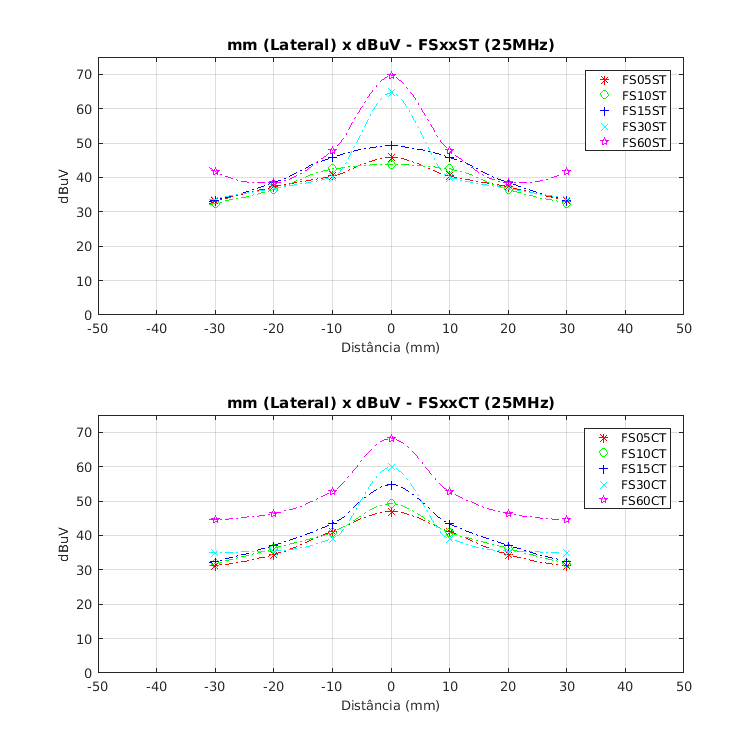
\includegraphics[scale=0.4]{./img/FSxxxT_25M}
		\label{fig:FSxxxT_25M}}
	\subfloat[][NFPs Face Dupla - 25MHz]{
		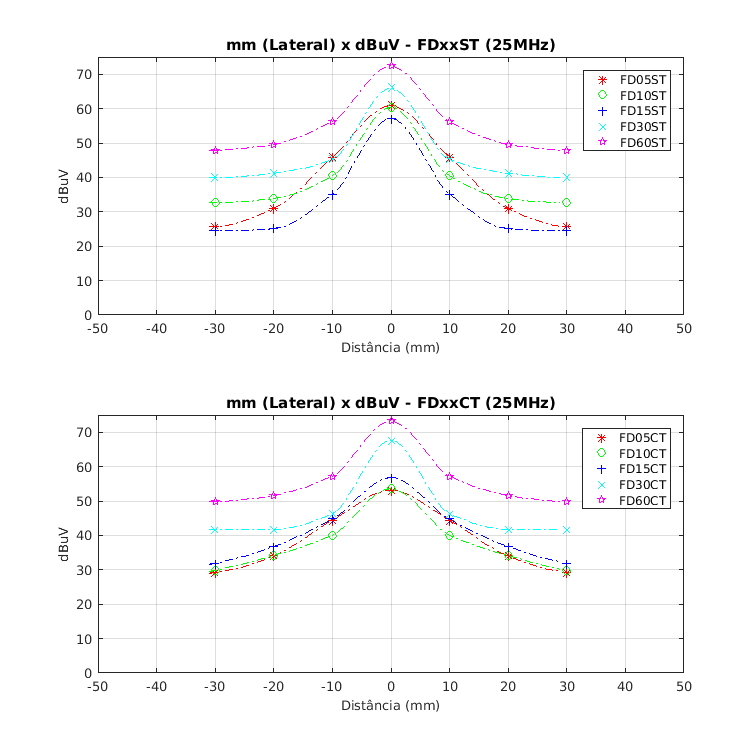
\includegraphics[scale=0.4]{./img/FDxxxT_25M}
		\label{fig:FDxxxT_25M}}
    \fonte{Elaborado pelo Autor (2019)}
\end{figure}

Na figura~\ref{fig:FSxxxT_25M} vemos os gráficos na frequência de 25MHz de todas as versões em face simples, sem e com plano de terra. Nesta imagem, no primeiro quadro, novamente exceto as versões FS30ST e FS60ST, todas as demais tem baixa sensibilidade e pouca resolução espacial, somente as versões FS30ST e FS60ST, que já possuem um raio maior que 1.5mm são as que apresentam uma boa sensibilidade nesta frequência. No segundo quadro da figura~\ref{fig:FSxxxT_25M}, com a inclusão do plano de terra, notamos que todas as versões melhoram sua sensibilidade, e notamos também que a versão FD60CT perde resolução espacial, haja vista que para todas as posições avaliadas esta versão possui um nível de tensão em $dB \mu V$ maior que as demais. 

Por fim, na figura~\ref{fig:FDxxxT_25M} vemos os gráficos na frequência de 25MHz de todas as versões em face dupla, sem e com plano de terra. Notamos no primeiro quadro desta imagem que o acréscimo de mais uma volta de espira aumente a sensibilidade para todas as versões de NFP avaliada, sendo que a que possui a melhor resolução espacial, nesta frequência, continuar sendo a FD15ST, mesmo tendo a menor sensibilidade. No segundo quadro da figura~\ref{fig:FDxxxT_25M} notamos que a inclusão do plano de terra, para esta frequência, não melhora a resolução espacial e não influência de forma significativa a sensibilidade. Dessa forma, o melhor resultado em termos de resolução espacial, nesta frequência (25MHz), assim como foi nas anteriores, é a versão FD15ST.

%###########################
%###########################

\section{Resultados da Caracterização da Resolução Espacial}
Conforme o procedimento descrito no capítulo anterior, realizou-se a captura da intensidade de tensão na NFP em $dB \mu V$ agora com dois DUTs operando simultaneamente, afim de verificar a distinção de cada frequência em posições espaciais diferentes. Estes resultados nos trazem uma melhor noção de resolução espacial e distinção de diferentes frequências.

\begin{figure}[htb!]
	\centering 
	\caption{Intensidades por Distâncias - NFPs Face Simples}
	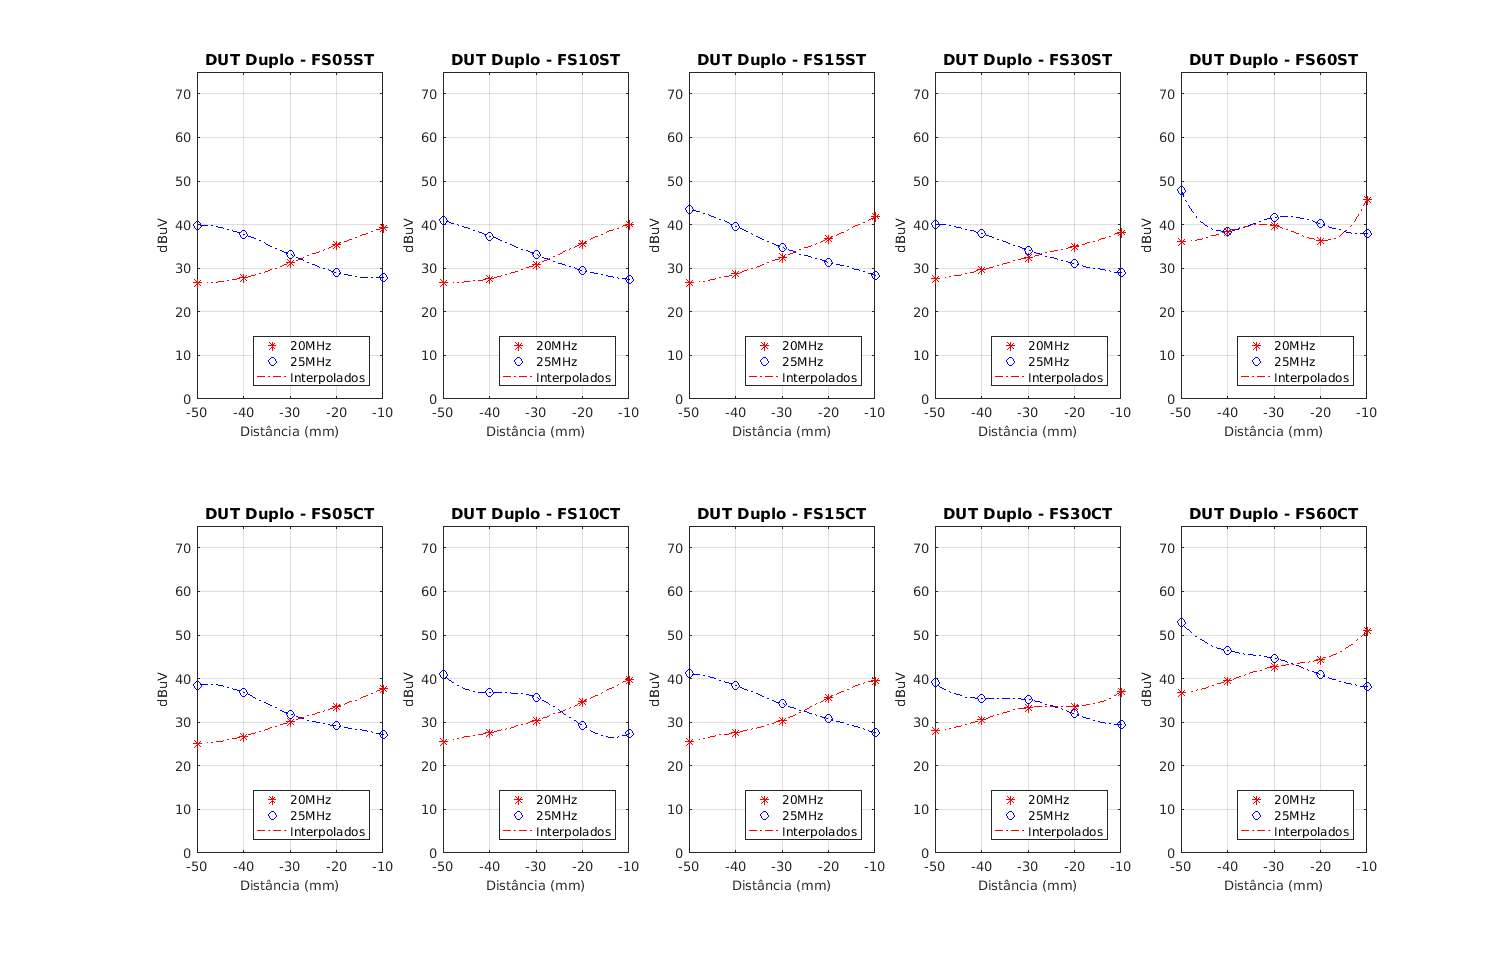
\includegraphics[scale=0.45]{./img/DUTDuplo_FS}
	\fonte{Elaborado pelo Autor (2019)}
	%\legend{\hspace{-218pt}Fonte:~\citeonline[p.~8]{paul2006}}
	\label{fig:DUTDuplo_FS}
\end{figure}

Na figura~\ref{fig:DUTDuplo_FS} visualizamos as medidas coletadas para todas as versões face simples, sendo que nos quadros da primeira fileira visualizamos as versões sem plano de terra e na fileira inferior visualizamos as versões com plano de terra. No primeiro quadro visualizamos as medidas coletadas para a NFP FS05ST e logo abaixo sua versão com plano de terra FS05CT, notamos que ambas as versões possuem respostas similares quanto a resolução espacial e distinção das frequências. No quadro que mostra a NFP FS30CT notamos uma leve diferenciação das frequências, porém é no caso FS60ST apresenta a melhor resolução espacial, porém em todas as posições são lidos valores mais altos de tensão em $dB \mu V$ do que as demais NFPs, mostrando que esta NFP é mais sensitiva do que as demais.

\begin{figure}[htb!]
	\centering 
	\caption{Intensidades por Distâncias - NFPs Face Simples}
	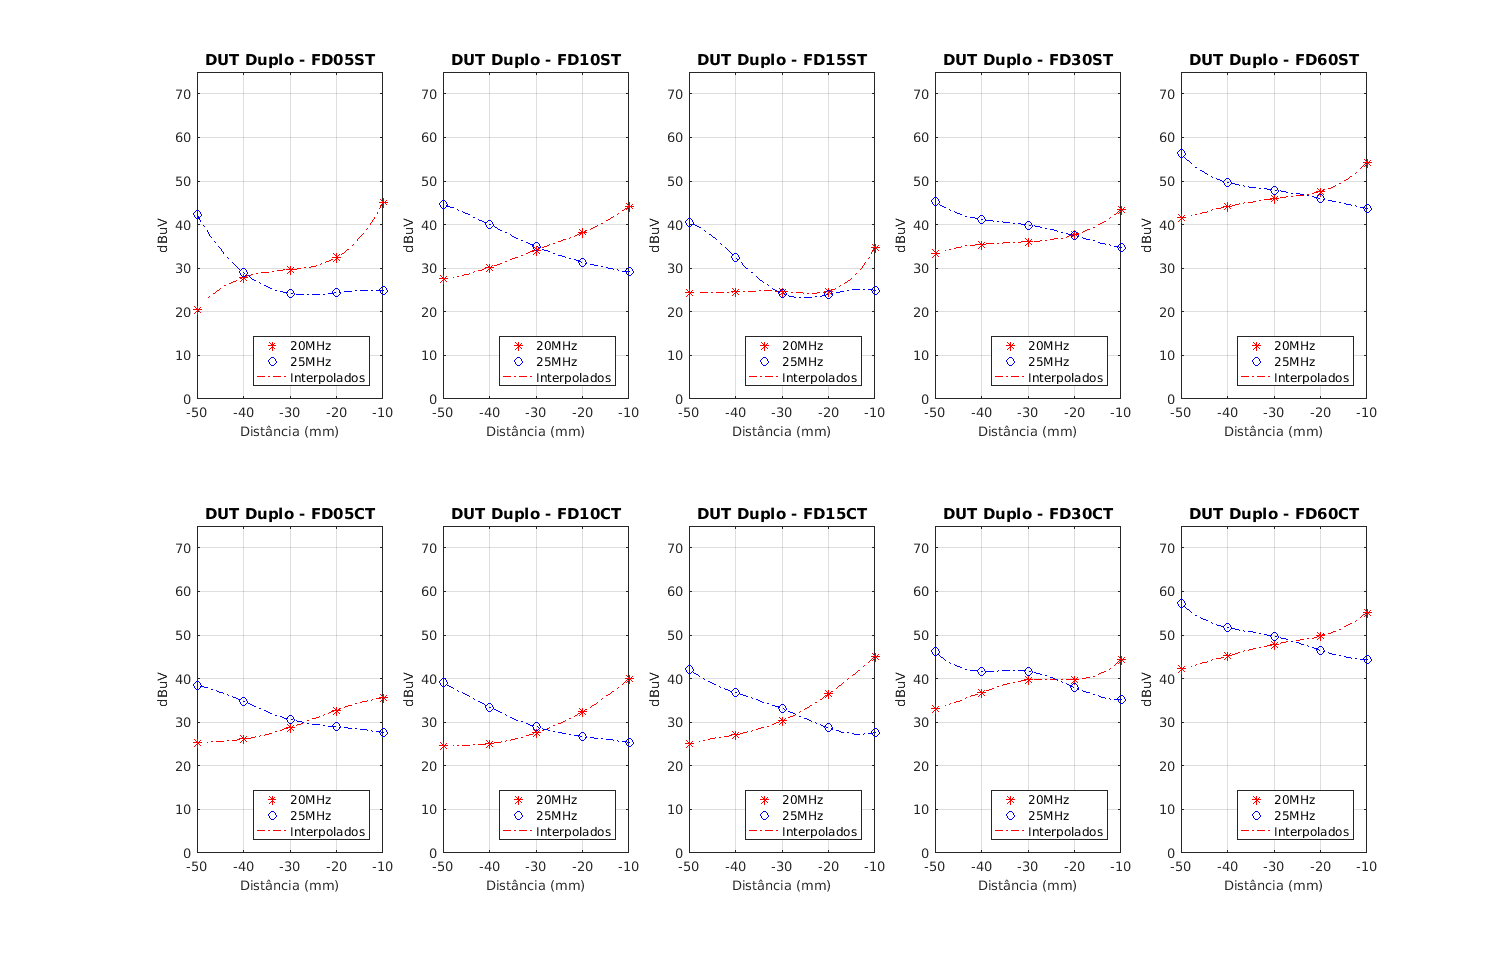
\includegraphics[scale=0.45]{./img/DUTDuplo_FD}
	\fonte{Elaborado pelo Autor (2019)}
	%\legend{\hspace{-218pt}Fonte:~\citeonline[p.~8]{paul2006}}
	\label{fig:DUTDuplo_FD}
\end{figure}

Na figura~\ref{fig:DUTDuplo_FD} visualizamos as medidas coletadas para todas as versões face dupla, sendo que nos quadros da primeira fileira visualizamos as versões sem plano de terra e na fileira inferior visualizamos as versões com plano de terra. No primeiro quadro visualizamos as medidas coletadas para a NFP FD05ST e logo abaixo sua versão com plano de terra FD05CT, aqui ja notamos uma boa resolução espacial para a FD05ST - lembramos aqui que esta NFP é a versão que ficou em um formato elíptico, isso pode ter influenciado neste resultado. Outra evidência clara que notamos é no quadro da FD15ST, que confirma que esta NFP tem uma boa resolução espacial, ficando assim de acordo com as medidas efetuadas na caracterização da intensidade por distância, exposta na última seção deste capítulo. Notamos também que as versões FD60ST e FD60CT também apresentam uma boa resolução espacial, porém estas NFPs são mais sensitivas que as demais, fornecendo valores de tensão em $dB \mu V$ em todas as posições avaliadas.

%###########################
%###########################

%\section{Melhores Resultados}

